% TikZ code for side-by-side dual proof sketch (v8 - simplified).
\begin{tikzpicture}[scale=0.8, every node/.style={transform shape, scale=0.8}]
% === BASE GRAPHS (H and H') ===
\uncover<1->{
\begin{scope}
\node at (-6, 3.5) {\huge$H$};
\coordinate (A1) at (-4.5, 6);
\coordinate (A2) at (-1.5, 8);
\coordinate (A3) at (1.5, 10);
\coordinate (B1) at (-4.5, 1);
\coordinate (B2) at (-1.5, -1);
\coordinate (B3) at (1.5, -3.2);
\coordinate (C1) at (6.5, 1.85);
\coordinate (C2) at (6.5, 6);
\coordinate (C3) at (7.5, 4.1);
\coordinate (R0) at (-2.3000000000000003, 3.0709999999999997);
\fill[gray!40] (R0) circle (2.0pt);
\draw[gray!40, line width=1.0pt] (R0) -- (A1);
\draw[gray!40, line width=1.0pt] (R0) -- (B1);
\draw[gray!40, line width=1.0pt] (R0) -- (C1);
\coordinate (R1) at (-2.3000000000000003, 4.15);
\fill[gray!40] (R1) circle (2.0pt);
\draw[gray!40, line width=1.0pt] (R1) -- (A1);
\draw[gray!40, line width=1.0pt] (R1) -- (B1);
\draw[gray!40, line width=1.0pt] (R1) -- (C2);
\coordinate (R2) at (-1.1000000000000005, 2.3309999999999995);
\fill[gray!40] (R2) circle (2.0pt);
\draw[gray!40, line width=1.0pt] (R2) -- (A1);
\draw[gray!40, line width=1.0pt] (R2) -- (B2);
\draw[gray!40, line width=1.0pt] (R2) -- (C1);
\coordinate (R3) at (-1.1000000000000005, 3.4099999999999997);
\fill[gray!40] (R3) circle (2.0pt);
\draw[gray!40, line width=1.0pt] (R3) -- (A1);
\draw[gray!40, line width=1.0pt] (R3) -- (B2);
\draw[gray!40, line width=1.0pt] (R3) -- (C2);
\coordinate (R4) at (-1.1000000000000005, 3.811);
\fill[gray!40] (R4) circle (2.0pt);
\draw[gray!40, line width=1.0pt] (R4) -- (A2);
\draw[gray!40, line width=1.0pt] (R4) -- (B1);
\draw[gray!40, line width=1.0pt] (R4) -- (C1);
\coordinate (R5) at (-1.1000000000000005, 4.890000000000001);
\fill[gray!40] (R5) circle (2.0pt);
\draw[gray!40, line width=1.0pt] (R5) -- (A2);
\draw[gray!40, line width=1.0pt] (R5) -- (B1);
\draw[gray!40, line width=1.0pt] (R5) -- (C2);
\coordinate (R6) at (0.09999999999999964, 3.0709999999999997);
\fill[gray!40] (R6) circle (2.0pt);
\draw[gray!40, line width=1.0pt] (R6) -- (A2);
\draw[gray!40, line width=1.0pt] (R6) -- (B2);
\draw[gray!40, line width=1.0pt] (R6) -- (C1);
\coordinate (R7) at (0.09999999999999964, 4.15);
\fill[gray!40] (R7) circle (2.0pt);
\draw[gray!40, line width=1.0pt] (R7) -- (A2);
\draw[gray!40, line width=1.0pt] (R7) -- (B2);
\draw[gray!40, line width=1.0pt] (R7) -- (C2);
\coordinate (R8) at (2.6999999999999997, 3.582);
\fill[gray!40] (R8) circle (2.0pt);
\draw[gray!40, line width=1.0pt] (R8) -- (A3);
\draw[gray!40, line width=1.0pt] (R8) -- (B3);
\draw[gray!40, line width=1.0pt] (R8) -- (C3);
\coordinate (R9) at (1.2999999999999998, 2.257);
\fill[gray!40] (R9) circle (2.0pt);
\draw[gray!40, line width=1.0pt] (R9) -- (A2);
\draw[gray!40, line width=1.0pt] (R9) -- (B3);
\draw[gray!40, line width=1.0pt] (R9) -- (C1);
\coordinate (R10) at (0.09999999999999987, 5.630000000000001);
\fill[gray!40] (R10) circle (2.0pt);
\draw[gray!40, line width=1.0pt] (R10) -- (A3);
\draw[gray!40, line width=1.0pt] (R10) -- (B1);
\draw[gray!40, line width=1.0pt] (R10) -- (C2);
\coordinate (R11) at (1.4999999999999996, 4.396);
\fill[gray!40] (R11) circle (2.0pt);
\draw[gray!40, line width=1.0pt] (R11) -- (A3);
\draw[gray!40, line width=1.0pt] (R11) -- (B2);
\draw[gray!40, line width=1.0pt] (R11) -- (C3);
\coordinate (R12) at (0.09999999999999987, 2.596);
\fill[gray!40] (R12) circle (2.0pt);
\draw[gray!40, line width=1.0pt] (R12) -- (A1);
\draw[gray!40, line width=1.0pt] (R12) -- (B3);
\draw[gray!40, line width=1.0pt] (R12) -- (C2);
\coordinate (R13) at (1.2999999999999998, 3.811);
\fill[gray!40] (R13) circle (2.0pt);
\draw[gray!40, line width=1.0pt] (R13) -- (A3);
\draw[gray!40, line width=1.0pt] (R13) -- (B2);
\draw[gray!40, line width=1.0pt] (R13) -- (C1);
\coordinate (R14) at (0.09999999999999987, 4.551);
\fill[gray!40] (R14) circle (2.0pt);
\draw[gray!40, line width=1.0pt] (R14) -- (A3);
\draw[gray!40, line width=1.0pt] (R14) -- (B1);
\draw[gray!40, line width=1.0pt] (R14) -- (C1);
\fill[black] (A1) circle (4.0pt) node[above=2pt, font=\Large] {$A_1$};
\fill[black] (A2) circle (4.0pt) node[above=2pt, font=\Large] {$A_2$};
\fill[black] (A3) circle (4.0pt) node[above=2pt, font=\Large] {$A_3$};
\fill[black] (B1) circle (4.0pt) node[right=2pt, font=\Large] {$B_1$};
\fill[black] (B2) circle (4.0pt) node[right=2pt, font=\Large] {$B_2$};
\fill[black] (B3) circle (4.0pt) node[right=2pt, font=\Large] {$B_3$};
\fill[black] (C1) circle (4.0pt) node[above=2pt, font=\Large] {$C_1$};
\fill[black] (C2) circle (4.0pt) node[above=2pt, font=\Large] {$C_2$};
\fill[black] (C3) circle (4.0pt) node[above=2pt, font=\Large] {$C_3$};
\end{scope}
\begin{scope}
\node at (21.5, 4) {\huge$H'$};
\coordinate (A1B1) at (13, 9.5);
\coordinate (A1B2) at (13, 8.0);
\coordinate (A1B3) at (13, 6.5);
\coordinate (A2B1) at (13, 5.0);
\coordinate (A2B2) at (13, 3.5);
\coordinate (A2B3) at (13, 2.0);
\coordinate (A3B1) at (13, 0.5);
\coordinate (A3B2) at (13, -1.0);
\coordinate (A3B3) at (13, -2.5);
\coordinate (C1HP) at (19, 7);
\coordinate (C2HP) at (19, 4);
\coordinate (C3HP) at (19, 1);
\node[anchor=south] at (13, 10) { \huge $U = V_1 \times V_2$ }; 
\node[anchor=south] at (19, 8.5) { \huge $W = V_3$};
\draw[line width=0.5pt, black!30] (A1B1) -- (C1HP);
\draw[line width=0.5pt, black!30] (A1B1) -- (C2HP);
\draw[line width=0.5pt, black!30] (A1B2) -- (C1HP);
\draw[line width=0.5pt, black!30] (A1B2) -- (C2HP);
\draw[line width=0.5pt, black!30] (A1B3) -- (C2HP);
\draw[line width=0.5pt, black!30] (A2B1) -- (C1HP);
\draw[line width=0.5pt, black!30] (A2B1) -- (C2HP);
\draw[line width=0.5pt, black!30] (A2B2) -- (C1HP);
\draw[line width=0.5pt, black!30] (A2B2) -- (C2HP);
\draw[line width=0.5pt, black!30] (A2B3) -- (C1HP);
\draw[line width=0.5pt, black!30] (A3B1) -- (C1HP);
\draw[line width=0.5pt, black!30] (A3B1) -- (C2HP);
\draw[line width=0.5pt, black!30] (A3B2) -- (C1HP);
\draw[line width=0.5pt, black!30] (A3B2) -- (C3HP);
\draw[line width=0.5pt, black!30] (A3B3) -- (C3HP);
\fill[black] (A1B1) circle (4.0pt) node[anchor=east, font=\Large, xshift=-4pt] {$(A_1,B_1)$};
\fill[black] (A1B2) circle (4.0pt) node[anchor=east, font=\Large, xshift=-4pt] {$(A_1,B_2)$};
\fill[black] (A1B3) circle (4.0pt) node[anchor=east, font=\Large, xshift=-4pt] {$(A_1,B_3)$};
\fill[black] (A2B1) circle (4.0pt) node[anchor=east, font=\Large, xshift=-4pt] {$(A_2,B_1)$};
\fill[black] (A2B2) circle (4.0pt) node[anchor=east, font=\Large, xshift=-4pt] {$(A_2,B_2)$};
\fill[black] (A2B3) circle (4.0pt) node[anchor=east, font=\Large, xshift=-4pt] {$(A_2,B_3)$};
\fill[black] (A3B1) circle (4.0pt) node[anchor=east, font=\Large, xshift=-4pt] {$(A_3,B_1)$};
\fill[black] (A3B2) circle (4.0pt) node[anchor=east, font=\Large, xshift=-4pt] {$(A_3,B_2)$};
\fill[black] (A3B3) circle (4.0pt) node[anchor=east, font=\Large, xshift=-4pt] {$(A_3,B_3)$};
\fill[black] (C1HP) circle (4.0pt) node[anchor=west, font=\Large, xshift=4pt] {$C_1$};
\fill[black] (C2HP) circle (4.0pt) node[anchor=west, font=\Large, xshift=4pt] {$C_2$};
\fill[black] (C3HP) circle (4.0pt) node[anchor=west, font=\Large, xshift=4pt] {$C_3$};
\end{scope}
}

% --- Link for C1 (Slide 2) ---
\only<2>{
\fill[blue] (R0) circle (2.0pt);
\draw[blue, line width=1.5pt] (R0) -- (A1);
\draw[blue, line width=1.5pt] (R0) -- (B1);
\draw[blue, line width=1.5pt] (R0) -- (C1);
\fill[blue] (R2) circle (2.0pt);
\draw[blue, line width=1.5pt] (R2) -- (A1);
\draw[blue, line width=1.5pt] (R2) -- (B2);
\draw[blue, line width=1.5pt] (R2) -- (C1);
\fill[blue] (R4) circle (2.0pt);
\draw[blue, line width=1.5pt] (R4) -- (A2);
\draw[blue, line width=1.5pt] (R4) -- (B1);
\draw[blue, line width=1.5pt] (R4) -- (C1);
\fill[blue] (R6) circle (2.0pt);
\draw[blue, line width=1.5pt] (R6) -- (A2);
\draw[blue, line width=1.5pt] (R6) -- (B2);
\draw[blue, line width=1.5pt] (R6) -- (C1);
\fill[blue] (R9) circle (2.0pt);
\draw[blue, line width=1.5pt] (R9) -- (A2);
\draw[blue, line width=1.5pt] (R9) -- (B3);
\draw[blue, line width=1.5pt] (R9) -- (C1);
\fill[blue] (R13) circle (2.0pt);
\draw[blue, line width=1.5pt] (R13) -- (A3);
\draw[blue, line width=1.5pt] (R13) -- (B2);
\draw[blue, line width=1.5pt] (R13) -- (C1);
\fill[blue] (R14) circle (2.0pt);
\draw[blue, line width=1.5pt] (R14) -- (A3);
\draw[blue, line width=1.5pt] (R14) -- (B1);
\draw[blue, line width=1.5pt] (R14) -- (C1);
\fill[blue] (C1) circle (4.5pt);
\begin{scope}
\fill[blue] (C1HP) circle (4.5pt);
\draw[line width=1.3pt, blue] (A1B1) -- (C1HP);
\fill[blue] (A1B1) circle (4.5pt);
\draw[line width=1.3pt, blue] (A1B2) -- (C1HP);
\fill[blue] (A1B2) circle (4.5pt);
\draw[line width=1.3pt, blue] (A2B1) -- (C1HP);
\fill[blue] (A2B1) circle (4.5pt);
\draw[line width=1.3pt, blue] (A2B2) -- (C1HP);
\fill[blue] (A2B2) circle (4.5pt);
\draw[line width=1.3pt, blue] (A2B3) -- (C1HP);
\fill[blue] (A2B3) circle (4.5pt);
\draw[line width=1.3pt, blue] (A3B1) -- (C1HP);
\fill[blue] (A3B1) circle (4.5pt);
\draw[line width=1.3pt, blue] (A3B2) -- (C1HP);
\fill[blue] (A3B2) circle (4.5pt);
\end{scope}
}

% --- 2D Graph for L(C1) (Slide 3) ---
\only<3>{
\draw[line width=1.5pt, blue, bend left=20] (A1) to (B1);
\draw[line width=1.5pt, blue, bend left=20] (A3) to (B1);
\draw[line width=1.5pt, blue, bend left=20] (A2) to (B3);
\draw[line width=1.5pt, blue, bend left=20] (A2) to (B2);
\draw[line width=1.5pt, blue, bend left=20] (A1) to (B2);
\draw[line width=1.5pt, blue, bend left=20] (A2) to (B1);
\draw[line width=1.5pt, blue, bend left=20] (A3) to (B2);
\fill[blue] (A3) circle (4.5pt);
\fill[blue] (A1) circle (4.5pt);
\fill[blue] (A2) circle (4.5pt);
\fill[blue] (B2) circle (4.5pt);
\fill[blue] (B1) circle (4.5pt);
\fill[blue] (B3) circle (4.5pt);
\begin{scope}
\node[draw, thick, fill=blue!20, rounded corners] at (0, -2) {2-graph $L_H(C1)$};
\end{scope}
\begin{scope}
\fill[blue] (C1HP) circle (4.5pt);
\draw[line width=1.3pt, blue] (A1B1) -- (C1HP);
\fill[blue] (A1B1) circle (4.5pt);
\draw[line width=1.3pt, blue] (A1B2) -- (C1HP);
\fill[blue] (A1B2) circle (4.5pt);
\draw[line width=1.3pt, blue] (A2B1) -- (C1HP);
\fill[blue] (A2B1) circle (4.5pt);
\draw[line width=1.3pt, blue] (A2B2) -- (C1HP);
\fill[blue] (A2B2) circle (4.5pt);
\draw[line width=1.3pt, blue] (A2B3) -- (C1HP);
\fill[blue] (A2B3) circle (4.5pt);
\draw[line width=1.3pt, blue] (A3B1) -- (C1HP);
\fill[blue] (A3B1) circle (4.5pt);
\draw[line width=1.3pt, blue] (A3B2) -- (C1HP);
\fill[blue] (A3B2) circle (4.5pt);
\end{scope}
}

% --- Link for C2 (Slide 4) ---
\only<4>{
\fill[orange] (R1) circle (2.0pt);
\draw[orange, line width=1.5pt] (R1) -- (A1);
\draw[orange, line width=1.5pt] (R1) -- (B1);
\draw[orange, line width=1.5pt] (R1) -- (C2);
\fill[orange] (R3) circle (2.0pt);
\draw[orange, line width=1.5pt] (R3) -- (A1);
\draw[orange, line width=1.5pt] (R3) -- (B2);
\draw[orange, line width=1.5pt] (R3) -- (C2);
\fill[orange] (R5) circle (2.0pt);
\draw[orange, line width=1.5pt] (R5) -- (A2);
\draw[orange, line width=1.5pt] (R5) -- (B1);
\draw[orange, line width=1.5pt] (R5) -- (C2);
\fill[orange] (R7) circle (2.0pt);
\draw[orange, line width=1.5pt] (R7) -- (A2);
\draw[orange, line width=1.5pt] (R7) -- (B2);
\draw[orange, line width=1.5pt] (R7) -- (C2);
\fill[orange] (R10) circle (2.0pt);
\draw[orange, line width=1.5pt] (R10) -- (A3);
\draw[orange, line width=1.5pt] (R10) -- (B1);
\draw[orange, line width=1.5pt] (R10) -- (C2);
\fill[orange] (R12) circle (2.0pt);
\draw[orange, line width=1.5pt] (R12) -- (A1);
\draw[orange, line width=1.5pt] (R12) -- (B3);
\draw[orange, line width=1.5pt] (R12) -- (C2);
\fill[orange] (C2) circle (4.5pt);
\begin{scope}
\fill[orange] (C2HP) circle (4.5pt);
\draw[line width=1.3pt, orange] (A1B1) -- (C2HP);
\fill[orange] (A1B1) circle (4.5pt);
\draw[line width=1.3pt, orange] (A1B2) -- (C2HP);
\fill[orange] (A1B2) circle (4.5pt);
\draw[line width=1.3pt, orange] (A1B3) -- (C2HP);
\fill[orange] (A1B3) circle (4.5pt);
\draw[line width=1.3pt, orange] (A2B1) -- (C2HP);
\fill[orange] (A2B1) circle (4.5pt);
\draw[line width=1.3pt, orange] (A2B2) -- (C2HP);
\fill[orange] (A2B2) circle (4.5pt);
\draw[line width=1.3pt, orange] (A3B1) -- (C2HP);
\fill[orange] (A3B1) circle (4.5pt);
\end{scope}
}

% --- 2D Graph for L(C2) (Slide 5) ---
\only<5>{
\draw[line width=1.5pt, orange, bend left=20] (A1) to (B1);
\draw[line width=1.5pt, orange, bend left=20] (A3) to (B1);
\draw[line width=1.5pt, orange, bend left=20] (A1) to (B3);
\draw[line width=1.5pt, orange, bend left=20] (A2) to (B2);
\draw[line width=1.5pt, orange, bend left=20] (A1) to (B2);
\draw[line width=1.5pt, orange, bend left=20] (A2) to (B1);
\fill[orange] (A3) circle (4.5pt);
\fill[orange] (A1) circle (4.5pt);
\fill[orange] (A2) circle (4.5pt);
\fill[orange] (B2) circle (4.5pt);
\fill[orange] (B1) circle (4.5pt);
\fill[orange] (B3) circle (4.5pt);
\begin{scope}
\node[draw, thick, fill=orange!20, rounded corners] at (0, -2) {2-graph $L_H(C2)$};
\end{scope}
\begin{scope}
\fill[orange] (C2HP) circle (4.5pt);
\draw[line width=1.3pt, orange] (A1B1) -- (C2HP);
\fill[orange] (A1B1) circle (4.5pt);
\draw[line width=1.3pt, orange] (A1B2) -- (C2HP);
\fill[orange] (A1B2) circle (4.5pt);
\draw[line width=1.3pt, orange] (A1B3) -- (C2HP);
\fill[orange] (A1B3) circle (4.5pt);
\draw[line width=1.3pt, orange] (A2B1) -- (C2HP);
\fill[orange] (A2B1) circle (4.5pt);
\draw[line width=1.3pt, orange] (A2B2) -- (C2HP);
\fill[orange] (A2B2) circle (4.5pt);
\draw[line width=1.3pt, orange] (A3B1) -- (C2HP);
\fill[orange] (A3B1) circle (4.5pt);
\end{scope}
}

% --- Link for C3 (Slide 6) ---
\only<6>{
\fill[green!50!black] (R8) circle (2.0pt);
\draw[green!50!black, line width=1.5pt] (R8) -- (A3);
\draw[green!50!black, line width=1.5pt] (R8) -- (B3);
\draw[green!50!black, line width=1.5pt] (R8) -- (C3);
\fill[green!50!black] (R11) circle (2.0pt);
\draw[green!50!black, line width=1.5pt] (R11) -- (A3);
\draw[green!50!black, line width=1.5pt] (R11) -- (B2);
\draw[green!50!black, line width=1.5pt] (R11) -- (C3);
\fill[green!50!black] (C3) circle (4.5pt);
\begin{scope}
\fill[green!50!black] (C3HP) circle (4.5pt);
\draw[line width=1.3pt, green!50!black] (A3B2) -- (C3HP);
\fill[green!50!black] (A3B2) circle (4.5pt);
\draw[line width=1.3pt, green!50!black] (A3B3) -- (C3HP);
\fill[green!50!black] (A3B3) circle (4.5pt);
\end{scope}
}

% --- 2D Graph for L(C3) (Slide 7) ---
\only<7>{
\draw[line width=1.5pt, green!50!black, bend left=20] (A3) to (B2);
\draw[line width=1.5pt, green!50!black, bend left=20] (A3) to (B3);
\fill[green!50!black] (A3) circle (4.5pt);
\fill[green!50!black] (B2) circle (4.5pt);
\fill[green!50!black] (B3) circle (4.5pt);
\begin{scope}
\node[draw, thick, fill=green!50!black!20, rounded corners] at (0, -2) {2-graph $L_H(C3)$};
\end{scope}
\begin{scope}
\fill[green!50!black] (C3HP) circle (4.5pt);
\draw[line width=1.3pt, green!50!black] (A3B2) -- (C3HP);
\fill[green!50!black] (A3B2) circle (4.5pt);
\draw[line width=1.3pt, green!50!black] (A3B3) -- (C3HP);
\fill[green!50!black] (A3B3) circle (4.5pt);
\end{scope}
}

% --- Common Link for T={C1, C2} (Slide 8) ---
\only<8>{
\fill[teal] (R0) circle (2.0pt);
\draw[teal, line width=1.5pt] (R0) -- (A1);
\draw[teal, line width=1.5pt] (R0) -- (B1);
\draw[teal, line width=1.5pt] (R0) -- (C1);
\fill[teal] (R1) circle (2.0pt);
\draw[teal, line width=1.5pt] (R1) -- (A1);
\draw[teal, line width=1.5pt] (R1) -- (B1);
\draw[teal, line width=1.5pt] (R1) -- (C2);
\fill[teal] (R2) circle (2.0pt);
\draw[teal, line width=1.5pt] (R2) -- (A1);
\draw[teal, line width=1.5pt] (R2) -- (B2);
\draw[teal, line width=1.5pt] (R2) -- (C1);
\fill[teal] (R3) circle (2.0pt);
\draw[teal, line width=1.5pt] (R3) -- (A1);
\draw[teal, line width=1.5pt] (R3) -- (B2);
\draw[teal, line width=1.5pt] (R3) -- (C2);
\fill[teal] (R4) circle (2.0pt);
\draw[teal, line width=1.5pt] (R4) -- (A2);
\draw[teal, line width=1.5pt] (R4) -- (B1);
\draw[teal, line width=1.5pt] (R4) -- (C1);
\fill[teal] (R5) circle (2.0pt);
\draw[teal, line width=1.5pt] (R5) -- (A2);
\draw[teal, line width=1.5pt] (R5) -- (B1);
\draw[teal, line width=1.5pt] (R5) -- (C2);
\fill[teal] (R6) circle (2.0pt);
\draw[teal, line width=1.5pt] (R6) -- (A2);
\draw[teal, line width=1.5pt] (R6) -- (B2);
\draw[teal, line width=1.5pt] (R6) -- (C1);
\fill[teal] (R7) circle (2.0pt);
\draw[teal, line width=1.5pt] (R7) -- (A2);
\draw[teal, line width=1.5pt] (R7) -- (B2);
\draw[teal, line width=1.5pt] (R7) -- (C2);
\fill[teal] (R10) circle (2.0pt);
\draw[teal, line width=1.5pt] (R10) -- (A3);
\draw[teal, line width=1.5pt] (R10) -- (B1);
\draw[teal, line width=1.5pt] (R10) -- (C2);
\fill[teal] (R14) circle (2.0pt);
\draw[teal, line width=1.5pt] (R14) -- (A3);
\draw[teal, line width=1.5pt] (R14) -- (B1);
\draw[teal, line width=1.5pt] (R14) -- (C1);
\fill[teal] (C1) circle (4.5pt);
\fill[teal] (C2) circle (4.5pt);
\fill[teal] (A1) circle (4.5pt);
\fill[teal] (B1) circle (4.5pt);
\fill[teal] (A1) circle (4.5pt);
\fill[teal] (B2) circle (4.5pt);
\fill[teal] (A2) circle (4.5pt);
\fill[teal] (B1) circle (4.5pt);
\fill[teal] (A2) circle (4.5pt);
\fill[teal] (B2) circle (4.5pt);
\fill[teal] (A3) circle (4.5pt);
\fill[teal] (B1) circle (4.5pt);
\begin{scope}
\fill[teal] (A1B1) circle (4.5pt);
\draw[line width=1.3pt, teal] (A1B1) -- (C1HP);
\draw[line width=1.3pt, teal] (A1B1) -- (C2HP);
\fill[teal] (A1B2) circle (4.5pt);
\draw[line width=1.3pt, teal] (A1B2) -- (C1HP);
\draw[line width=1.3pt, teal] (A1B2) -- (C2HP);
\fill[teal] (A2B1) circle (4.5pt);
\draw[line width=1.3pt, teal] (A2B1) -- (C1HP);
\draw[line width=1.3pt, teal] (A2B1) -- (C2HP);
\fill[teal] (A2B2) circle (4.5pt);
\draw[line width=1.3pt, teal] (A2B2) -- (C1HP);
\draw[line width=1.3pt, teal] (A2B2) -- (C2HP);
\fill[teal] (A3B1) circle (4.5pt);
\draw[line width=1.3pt, teal] (A3B1) -- (C1HP);
\draw[line width=1.3pt, teal] (A3B1) -- (C2HP);
\fill[teal] (C1HP) circle (4.5pt);
\fill[teal] (C2HP) circle (4.5pt);
\end{scope}
}

% --- 2D Graph for L(T) (Slide 9) ---
\only<9>{
\draw[line width=1.5pt, teal, bend left=20] (A1) to (B1);
\draw[line width=1.5pt, teal, bend left=20] (A3) to (B1);
\draw[line width=1.5pt, teal, bend left=20] (A2) to (B2);
\draw[line width=1.5pt, teal, bend left=20] (A1) to (B2);
\draw[line width=1.5pt, teal, bend left=20] (A2) to (B1);
\fill[teal] (A3) circle (4.5pt);
\fill[teal] (A1) circle (4.5pt);
\fill[teal] (A2) circle (4.5pt);
\fill[teal] (B2) circle (4.5pt);
\fill[teal] (B1) circle (4.5pt);
\node[draw, thick, fill=teal!20, rounded corners] at (0, -2) {2-graph $L_H(T)$};
\begin{scope}
\fill[teal] (A1B1) circle (4.5pt);
\draw[line width=1.3pt, teal] (A1B1) -- (C1HP);
\draw[line width=1.3pt, teal] (A1B1) -- (C2HP);
\fill[teal] (A1B2) circle (4.5pt);
\draw[line width=1.3pt, teal] (A1B2) -- (C1HP);
\draw[line width=1.3pt, teal] (A1B2) -- (C2HP);
\fill[teal] (A2B1) circle (4.5pt);
\draw[line width=1.3pt, teal] (A2B1) -- (C1HP);
\draw[line width=1.3pt, teal] (A2B1) -- (C2HP);
\fill[teal] (A2B2) circle (4.5pt);
\draw[line width=1.3pt, teal] (A2B2) -- (C1HP);
\draw[line width=1.3pt, teal] (A2B2) -- (C2HP);
\fill[teal] (A3B1) circle (4.5pt);
\draw[line width=1.3pt, teal] (A3B1) -- (C1HP);
\draw[line width=1.3pt, teal] (A3B1) -- (C2HP);
\fill[teal] (C1HP) circle (4.5pt);
\fill[teal] (C2HP) circle (4.5pt);
\end{scope}
}

% --- Found K(2,2) in L(T) (Slide 10) ---
\only<10>{
\draw[line width=1.5pt, teal!40, bend left=20] (A1) to (B1);
\draw[line width=1.5pt, teal!40, bend left=20] (A3) to (B1);
\draw[line width=1.5pt, teal!40, bend left=20] (A2) to (B2);
\draw[line width=1.5pt, teal!40, bend left=20] (A1) to (B2);
\draw[line width=1.5pt, teal!40, bend left=20] (A2) to (B1);
\draw[line width=2pt, purple, bend left=20] (A1) to (B1);
\draw[line width=2pt, purple, bend left=20] (A1) to (B2);
\draw[line width=2pt, purple, bend left=20] (A2) to (B1);
\draw[line width=2pt, purple, bend left=20] (A2) to (B2);
\fill[purple] (A1) circle (4.5pt);
\fill[purple] (A2) circle (4.5pt);
\fill[purple] (B1) circle (4.5pt);
\fill[purple] (B2) circle (4.5pt);
\node[draw, thick, fill=purple!20, rounded corners] at (0, -2) {$K(2,2) \subset L_H(T)$};
\begin{scope}
\fill[teal] (A3B1) circle (4.5pt);
\draw[line width=1.3pt, teal] (A3B1) -- (C1HP);
\draw[line width=1.3pt, teal] (A3B1) -- (C2HP);
\fill[purple] (A1B1) circle (4.5pt);
\draw[line width=1.3pt, purple] (A1B1) -- (C1HP);
\draw[line width=1.3pt, purple] (A1B1) -- (C2HP);
\fill[purple] (A1B2) circle (4.5pt);
\draw[line width=1.3pt, purple] (A1B2) -- (C1HP);
\draw[line width=1.3pt, purple] (A1B2) -- (C2HP);
\fill[purple] (A2B1) circle (4.5pt);
\draw[line width=1.3pt, purple] (A2B1) -- (C1HP);
\draw[line width=1.3pt, purple] (A2B1) -- (C2HP);
\fill[purple] (A2B2) circle (4.5pt);
\draw[line width=1.3pt, purple] (A2B2) -- (C1HP);
\draw[line width=1.3pt, purple] (A2B2) -- (C2HP);
\fill[purple] (C1HP) circle (4.5pt);
\fill[purple] (C2HP) circle (4.5pt);
\end{scope}
}

% --- FINAL K(2,2,2) in H (Slide 11) ---
\only<11>{
\fill[brown!60!red] (R0) circle (2.5pt);
\draw[brown!60!red, line width=1.8pt] (R0) -- (A1);
\draw[brown!60!red, line width=1.8pt] (R0) -- (B1);
\draw[brown!60!red, line width=1.8pt] (R0) -- (C1);
\fill[brown!60!red] (R1) circle (2.5pt);
\draw[brown!60!red, line width=1.8pt] (R1) -- (A1);
\draw[brown!60!red, line width=1.8pt] (R1) -- (B1);
\draw[brown!60!red, line width=1.8pt] (R1) -- (C2);
\fill[brown!60!red] (R2) circle (2.5pt);
\draw[brown!60!red, line width=1.8pt] (R2) -- (A1);
\draw[brown!60!red, line width=1.8pt] (R2) -- (B2);
\draw[brown!60!red, line width=1.8pt] (R2) -- (C1);
\fill[brown!60!red] (R3) circle (2.5pt);
\draw[brown!60!red, line width=1.8pt] (R3) -- (A1);
\draw[brown!60!red, line width=1.8pt] (R3) -- (B2);
\draw[brown!60!red, line width=1.8pt] (R3) -- (C2);
\fill[brown!60!red] (R4) circle (2.5pt);
\draw[brown!60!red, line width=1.8pt] (R4) -- (A2);
\draw[brown!60!red, line width=1.8pt] (R4) -- (B1);
\draw[brown!60!red, line width=1.8pt] (R4) -- (C1);
\fill[brown!60!red] (R5) circle (2.5pt);
\draw[brown!60!red, line width=1.8pt] (R5) -- (A2);
\draw[brown!60!red, line width=1.8pt] (R5) -- (B1);
\draw[brown!60!red, line width=1.8pt] (R5) -- (C2);
\fill[brown!60!red] (R6) circle (2.5pt);
\draw[brown!60!red, line width=1.8pt] (R6) -- (A2);
\draw[brown!60!red, line width=1.8pt] (R6) -- (B2);
\draw[brown!60!red, line width=1.8pt] (R6) -- (C1);
\fill[brown!60!red] (R7) circle (2.5pt);
\draw[brown!60!red, line width=1.8pt] (R7) -- (A2);
\draw[brown!60!red, line width=1.8pt] (R7) -- (B2);
\draw[brown!60!red, line width=1.8pt] (R7) -- (C2);
\fill[brown!60!red] (A1) circle (4.5pt);
\fill[brown!60!red] (A2) circle (4.5pt);
\fill[brown!60!red] (B1) circle (4.5pt);
\fill[brown!60!red] (B2) circle (4.5pt);
\fill[brown!60!red] (C1) circle (4.5pt);
\fill[brown!60!red] (C2) circle (4.5pt);
\node[draw, thick, fill=brown!60!red!20, rounded corners, align=center] at (0, -2) {$K(2,2,2)$ found in $H$};
\begin{scope}
\fill[brown!60!red] (A1B1) circle (4.5pt);
\draw[line width=1.3pt, brown!60!red] (A1B1) -- (C1HP);
\draw[line width=1.3pt, brown!60!red] (A1B1) -- (C2HP);
\fill[brown!60!red] (A1B2) circle (4.5pt);
\draw[line width=1.3pt, brown!60!red] (A1B2) -- (C1HP);
\draw[line width=1.3pt, brown!60!red] (A1B2) -- (C2HP);
\fill[brown!60!red] (A2B1) circle (4.5pt);
\draw[line width=1.3pt, brown!60!red] (A2B1) -- (C1HP);
\draw[line width=1.3pt, brown!60!red] (A2B1) -- (C2HP);
\fill[brown!60!red] (A2B2) circle (4.5pt);
\draw[line width=1.3pt, brown!60!red] (A2B2) -- (C1HP);
\draw[line width=1.3pt, brown!60!red] (A2B2) -- (C2HP);
\fill[brown!60!red] (C1HP) circle (4.5pt);
\fill[brown!60!red] (C2HP) circle (4.5pt);
\end{scope}
}
\end{tikzpicture}